\documentclass[../main.tex]{subfiles}
\graphicspath{../images/}

\begin{document}
\section{Projekt produktu programowego}
    \subsection{Baza danych}
        Baza danych została zaimplementowana w PostgreSQL według diagramu na Rysunku \ref{fig:db-diagram}.

        \begin{figure}[H]
            \centering
            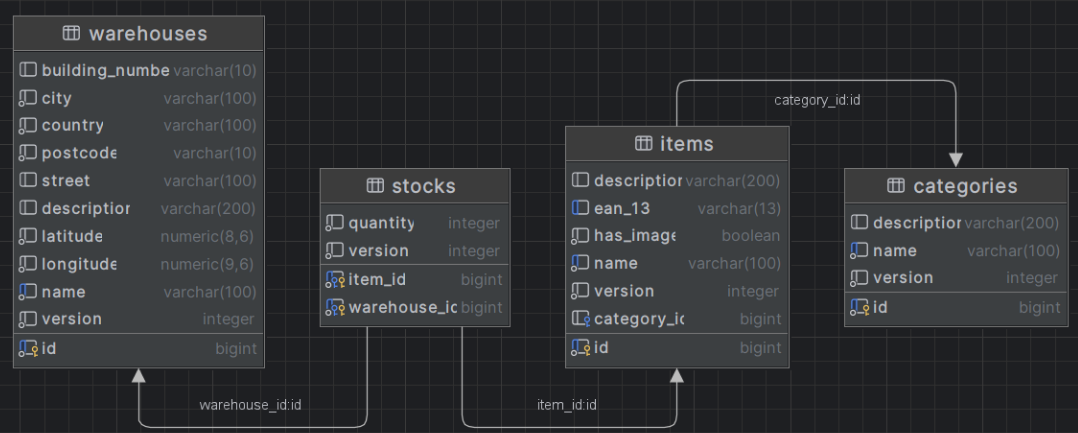
\includegraphics[width=1.0\linewidth]{images/db-diagram.png}
            \caption{Diagram reprezentujący fizyczny schemat bazy danych}
            \label{fig:db-diagram}
        \end{figure}

    \subsection{Architektura}
        Architektura aplikacji została wdrożona przy pomocy narzędzia HashiCorp Terraform na platformie AWS. Schemat zawierający najważniejsze elementy architektury przedstawiony jest na Rysunku \ref{fig:aws-architecture} 
        \begin{figure}[H]
            \centering
            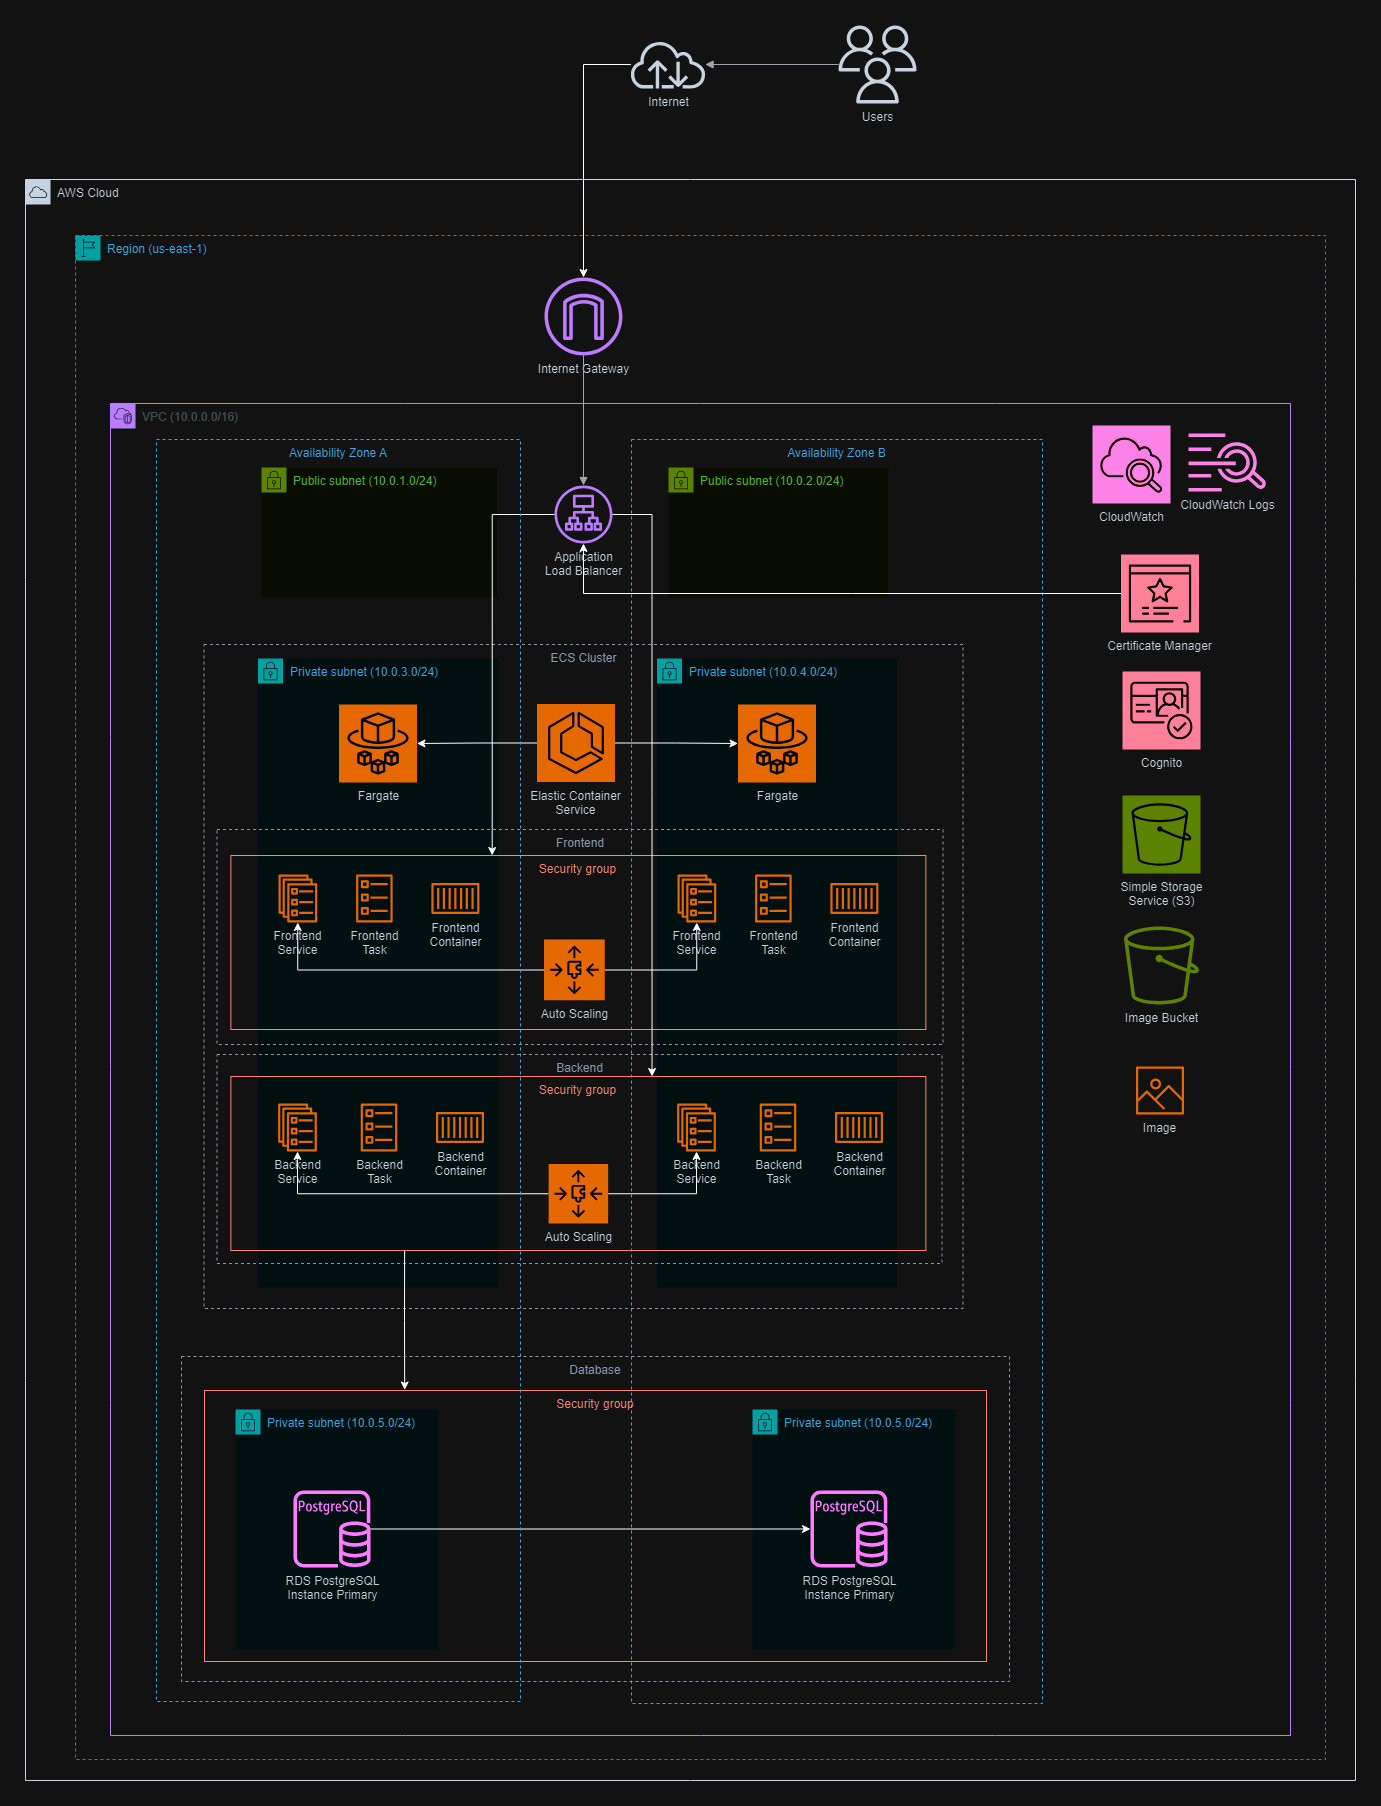
\includegraphics[width=1.0\linewidth]{images/AWS-diagram.png}
            \caption{Diagram architektury AWS}
            \label{fig:aws-architecture}
        \end{figure}

    \FloatBarrier
    \subsection{Pozostałe schematy i diagramy}

        \subsubsection*{Diagram wdrożenia systemu}
        Diagram UML wdrożenia aplikacji przedstawia abstrakcyjny zarys połączeń między kluczowymi elementami systemu, uwzględniając protokoły komunikacyjne i inne charakterystyczne elementy takie jak artefakty. Diagram przedstawiony jest na Rysunku \ref{fig:deployment-diagram}.
        \begin{figure}[H]
            \centering
            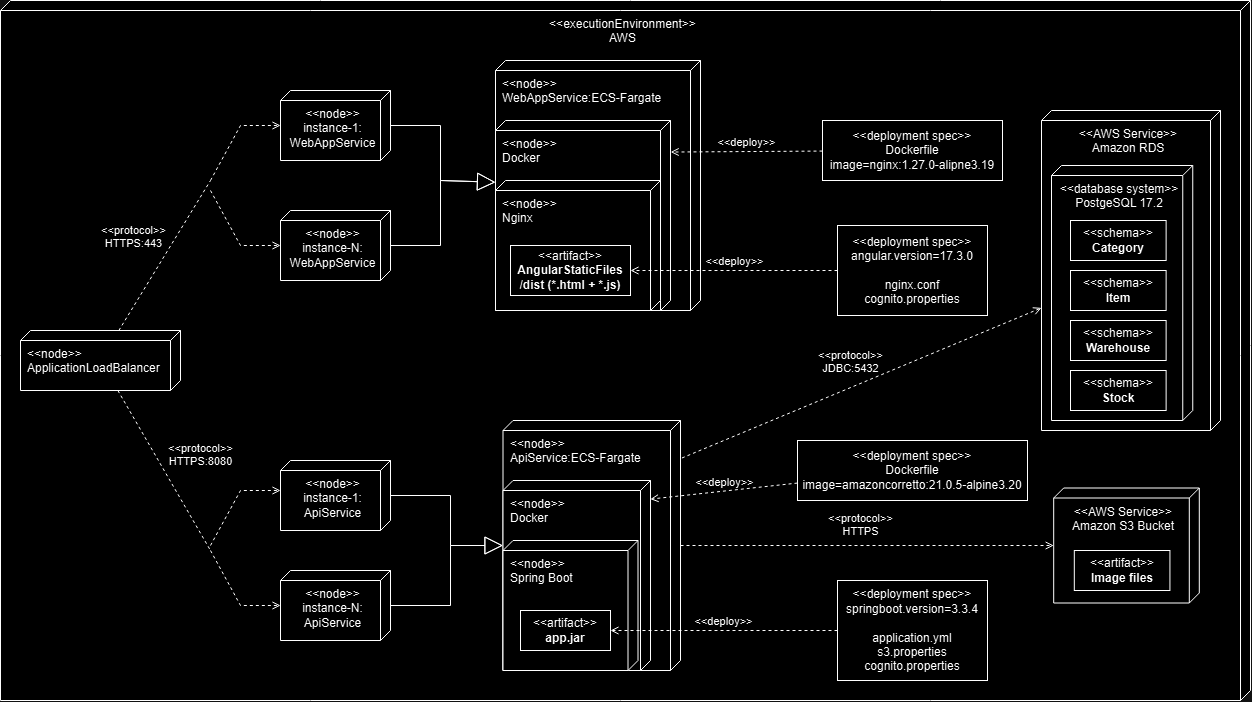
\includegraphics[width=1.0\linewidth]{images/deployment-diagram.png}
            \caption{Diagram wdrożenia systemu}
            \label{fig:deployment-diagram}
        \end{figure}

        % \subsubsection*{Diagram przypadków użycia}
        % \subsubsection*{Diagram klas}
        % \subsubsection*{Schemat przebiegu aplikacji}

\end{document}